\pdfvariable minorversion=7
\pdfvariable inclusioncopyfonts=1

\documentclass{arialFHGR} % use either arialFHGR or timesFHGR
\newcommand{\haupttitel}{Proposal Masterthesis}
\newcommand{\untertitel}{Interaktive Visualisierung dynamischer Netzwerke - Implementierung eines Visual Analytics Tools zur Exploration von Anomalien und Trends im SBB Zugverkehrsnetzwerk}
\newcommand{\zusammenfassung}{Abstract}
\newcommand{\autorenschaft}{Yannick Hutter}
\newcommand{\studiengang}{Msc User Experience Design \& Data Visualization}
\newcommand{\matrikelnummer}{17-175-829}
\newcommand{\adresse}{Talackerstrasse 8}
\newcommand{\ort}{Mels}
\newcommand{\plz}{8887}
\newcommand{\department}{[Departement]}
\newcommand{\institute}{[Institutsname]}
\newcommand{\modul}{Masterthesis FS25}
\newcommand{\email}{yannick.hutter@stud.fhgr.ch}
\newcommand{\refe}{Dr. rer. nat Michael Burch}
\newcommand{\coRefe}{Prof. Dr. habil. Wolfgang Semar}
\newcommand{\abgabedatum}{02.05.2025}
\newcommand{\abgabedatumRFC}{2025-05-02}
\newcommand{\sprache}{de}
\newcommand{\schlagworte}{}

\usepackage{setspace, fancyhdr, lscape, floatrow, caption, inputenc, graphicx, enumitem, tabularx, colorprofiles, xstring, hyphenat, chngcntr, xspace, listings, pdfpages}

\usepackage[left=3cm,right=2.5cm,top=2.5cm,bottom=2cm]{geometry}
\usepackage[backend=biber,style=apa,citestyle=apa]{biblatex}
\usepackage[autostyle]{csquotes}
\usepackage[english, nswissgerman]{babel}
\usepackage[titles]{tocloft}
\usepackage[hang,flushmargin]{footmisc}

% Settings for glossary
\usepackage[acronym,toc=true,xindy,nopostdot=true,nonumberlist,nogroupskip=true]{glossaries}
\loadglsentries{content/01_vorspann/01.4_abkuerzungsverzeichnis_glossar}
\setglossarystyle{alttree}
\setglossarypreamble[acronym]{\vspace*{-8pt}}
\makeglossaries
\glsaddall
\glsfindwidesttoplevelname

\graphicspath{{content/00_assets}} % Set path as default for including graphics
\addbibresource{content/00_assets/quellen.bib} % Add bibliography entries

% cite with acronym. 
% Example input: \citeAbbr{schweizerische_archivdirektorinnen-_und_archivdirektorenkonferenz_informations-_2018}{adk}
\newcommand{\parenciteabbr}[2]{(\acrlong{#2} [\acrshort{#2}], \citeyear{#1})}
\newcommand{\textciteabbr}[2]{\acrlong{#2} (\acrshort{#2}, \citeyear{#1})}
\newcommand{\acrfullSqBr}[1]{\acrlong{#1} [\acrshort{#1}]}

\setmonofont{Courier New}

% Settings for listings
\lstdefinestyle{codeStyle}{
    belowcaptionskip=6pt,
    belowskip=3pt,
    breaklines=true,
    numbers=left,
    basicstyle=\footnotesize\ttfamily,
    extendedchars=true,
    frame=single,
    captionpos=t,
    numberbychapter=false,
    xleftmargin=4pt,
    xrightmargin=4pt
}
\lstset{style=codeStyle}

% Settings for blockquote
\SetBlockEnvironment{quotation}
\patchcmd{\quotation}{\rightmargin}{\leftmargin 1.3cm \rightmargin 0}{}{}
\NewCommandCopy{\oldblockquote}{\blockquote}
\renewcommand{\blockquote}[1]{\oldblockquote{\noindent #1}}

% Settings for figure and table
\counterwithout{figure}{chapter}
\counterwithout{table}{chapter}

\floatsetup[figure]{
    capposition=above,
    captionskip=2pt
}

\DeclareCaptionLabelFormat{figTitle}{%
    Abbildung \the\numexpr\value{figure}\relax\\
}

\captionsetup[figure]{
    font={normalsize,stretch=1.0},
    labelfont=bf,
    labelsep=none,
    labelformat=figTitle,
    textfont=it,
    justification=raggedright,
    singlelinecheck=false,
    position=above,
}

\floatsetup[table]{
    capposition=above,
    captionskip=2pt
}

\DeclareCaptionLabelFormat{tabTitle}{%
    Tabelle \the\numexpr\value{table}\relax \\
} 

\captionsetup[table]{
    font={normalsize,stretch=1.0},
    labelfont={bf},
    labelsep=none,
    labelformat=tabTitle,
    textfont=it,
    justification=raggedright,
    singlelinecheck=false,
    position=above
}

\floatsetup[lstlisting]{
    capposition=above,
    captionskip=2pt
}

\DeclareCaptionLabelFormat{codeTitle}{%
    Programmcode \the\numexpr\value{lstlisting}\relax \\
} 

\captionsetup[lstlisting]{
    font={normalsize,stretch=1.0},
    labelfont={bf},
    labelsep=none,
    labelformat=codeTitle,
    textfont=it,
    justification=raggedright,
    singlelinecheck=false,
    position=above
}

\renewcommand{\thetable}{\arabic{table}}
\renewcommand{\thefigure}{\arabic{figure}}

% Einstellungen für tocloft / Settings for tocloft
\renewcommand{\cftfigpresnum}{Abb.~}
\renewcommand{\cfttabpresnum}{Tab.~}
\renewcommand{\cftfigaftersnum}{:}
\renewcommand{\cfttabaftersnum}{:}
\setlength{\cftfignumwidth}{2cm}
\setlength{\cfttabnumwidth}{2cm}
\setlength{\cftfigindent}{0cm}
\setlength{\cfttabindent}{0cm}

\setstretch{1.3} % Zeilenabstand / line spacing
\renewcommand{\arraystretch}{1.3} % Zeilenabstand innerhalb von Tabellen / line spacing in tables
\setlength{\parindent}{1.3cm} % Einzug neuer Absatz / Indentation new paragraph
\fancyhf{}
\renewcommand{\headrulewidth}{0pt}
\pagestyle{fancyplain}
\rfoot{\footnotesize\thepage}

\usepackage[pdfa]{hyperref}
\usepackage{hyperxmp}
\usepackage{embedfile}
\pdfvariable omitcidset=1

% 
\newcommand{\chapterNoNr}[1]{%
    \chapter*{#1}
    \addcontentsline{toc}{chapter}{#1} %
}%

\newcommand{\note}[1]{%
    \doublespacing\raggedright\footnotesize{\textit{Anmerkung:} #1}
}%

\newcommand{\sic}{%
    [\textit{sic}]\xspace
}%

\makeatletter
\def\l@lstlisting#1#2{\@dottedtocline{1}{0em}{2em}{Programmcode #1}{#2}}
\makeatother

\hypersetup{%
    pdflang=\sprache,
    pdftitle={\haupttitel},
    pdfsubtitle={\untertitel},
    pdfauthor={\autorenschaft},
    pdfdate={\abgabedatumRFC},
    pdfsubject={\zusammenfassung},
    pdfkeywords={\modul, \schlagworte},
    pdfcontactaddress={\adresse},
    pdfcontactcity={\ort},
    pdfcontactpostcode={\plz},
    pdfcontactemail={\email},
    colorlinks,
    unicode,
    allcolors=black,
    pdfapart=2,
    pdfaconformance=U
}

% 
\immediate\pdfobj stream attr{/N 3} file{sRGB.icc}
\pdfcatalog{%
  /OutputIntents [
    <<
      /Type /OutputIntent
      /S /GTS_PDFA1
      /DestOutputProfile \the\pdflastobj\space 0 R
      /OutputConditionIdentifier (sRGB)
      /Info (sRGB)
    >>
  ]
}

\begin{document}

    \renewcommand{\contentsname}{Inhaltsverzeichnis}
    \renewcommand{\listfigurename}{Abbildungsverzeichnis}
    \renewcommand{\listtablename}{Tabellenverzeichnis}
    \renewcommand{\acronymname}{Abkürzungsverzeichnis}
    \renewcommand{\lstlistlistingname}{\texorpdfstring{Programmcodeverzeichnis\bigskip}{Programmcodeverzeichnis}}
    
    % Start Vorspann
    
    \pagenumbering{Roman} % Begin roman pagenumbering

    % Titelblatt für eine Studienarbeit
     \begin{titlepage}
    
    \begin{center}
        Geschrieben an der Fachhochschule Graubünden \\
        \vspace{30mm}
        \huge\textbf{\haupttitel}\\
        \hfill \break
        \large{(\untertitel)}
    \end{center}
    
    \vfill
    
    \begin{flushleft}
    Name: \autorenschaft\\
    Studiengang: \studiengang\\
    Matrikelnummer: \matrikelnummer\\
    Adresse: \adresse, \plz~\ort\\
    E-Mail: \email\\
    ~\\
    Modul: \modul\\
    Referent: \refe\\
    Koreferent: \coRefe\\
    ~\\
    Abgabedatum: \abgabedatum
    \end{flushleft}
    
    \vspace{20mm}
    
\end{titlepage}

    % ODER für eine Abschlussarbeit
    % \begin{titlepage}
    \begin{center}
        {\large
            {\Large\textbf{\haupttitel}} \\
            \textit{\untertitel} \\
            ~\\
            An der Fachhochschule Graubünden \\
            \department \\
            \institute \\
            \vspace{2mm}
            im Studiengang \studiengang{} eingereichte \\
            ~\\
            {\Huge\textbf{Masterarbeit}} \\
            ~\\
            zur Erlangung des akademischen Grades \\
            eines Master of Science (M.Sc.)
    
            \vspace{40mm}
            vorgelegt von \\
            \vspace{4mm}
            {\Large\textbf{\autorenschaft}} \\
            \vspace{4mm}
            Matrikelnr.: \matrikelnummer \\
            E-Mail: \email \\
            ~\\~\\
            Erstgutachter: \refe \\
            Zweitgutachter: \coRefe \\
            ~\\
            Eingereicht am: \abgabedatum
        } % end large
    \end{center}
\end{titlepage}


    \include{content/01_vorspann/01.2_abstract}
    \include{content/01_vorspann/01.3_vorwort}

    \tableofcontents % Inhaltsverzeichnis
        
    % List of figures
    \cleardoublepage
    \phantomsection
    \addcontentsline{toc}{chapter}{\listfigurename}
    \listoffigures
    
    % List of tables
    \cleardoublepage
    \phantomsection
    \addcontentsline{toc}{chapter}{\listtablename}
    \listoftables

    % List of acronyms
    \printglossary[type=\acronymtype]
    \cleardoublepage
    \newpage
    % Ende Vorspann
    
    % Start Textteil
    \pagenumbering{arabic} % Begin arabic pagenumbering
    \include{content/02_textteil/einleitung}
    \chapter{Forschungsproblem und Forschungsziel}
\label{kap:forschungsproblem_forschungsziel}
Schweizer fahren gerne Zug, dies zeigt ein Artikel von Litra, welcher die Nutzung des Zuges in Europa untersuchte \parencite{litra_bahnfahrtstatistik_europa_2023}. Alleine im Jahr 2023 legten die Schweizer rund 2'466 Bahnkilometer pro Einwohner zurück (siehe Abbildung \ref{fig_schweizer_fahren_zug}). Dies entspricht einem Zuwachs von rund 13 Prozent im Vergleich zum Vorjahr. 

\begin{figure}[H]
    \caption{Zurückgelegte Kilometer pro Einwohnerin und Einwohner 2023 (Personenkilometer) \parencite{litra_bahnfahrtstatistik_europa_2023}}
    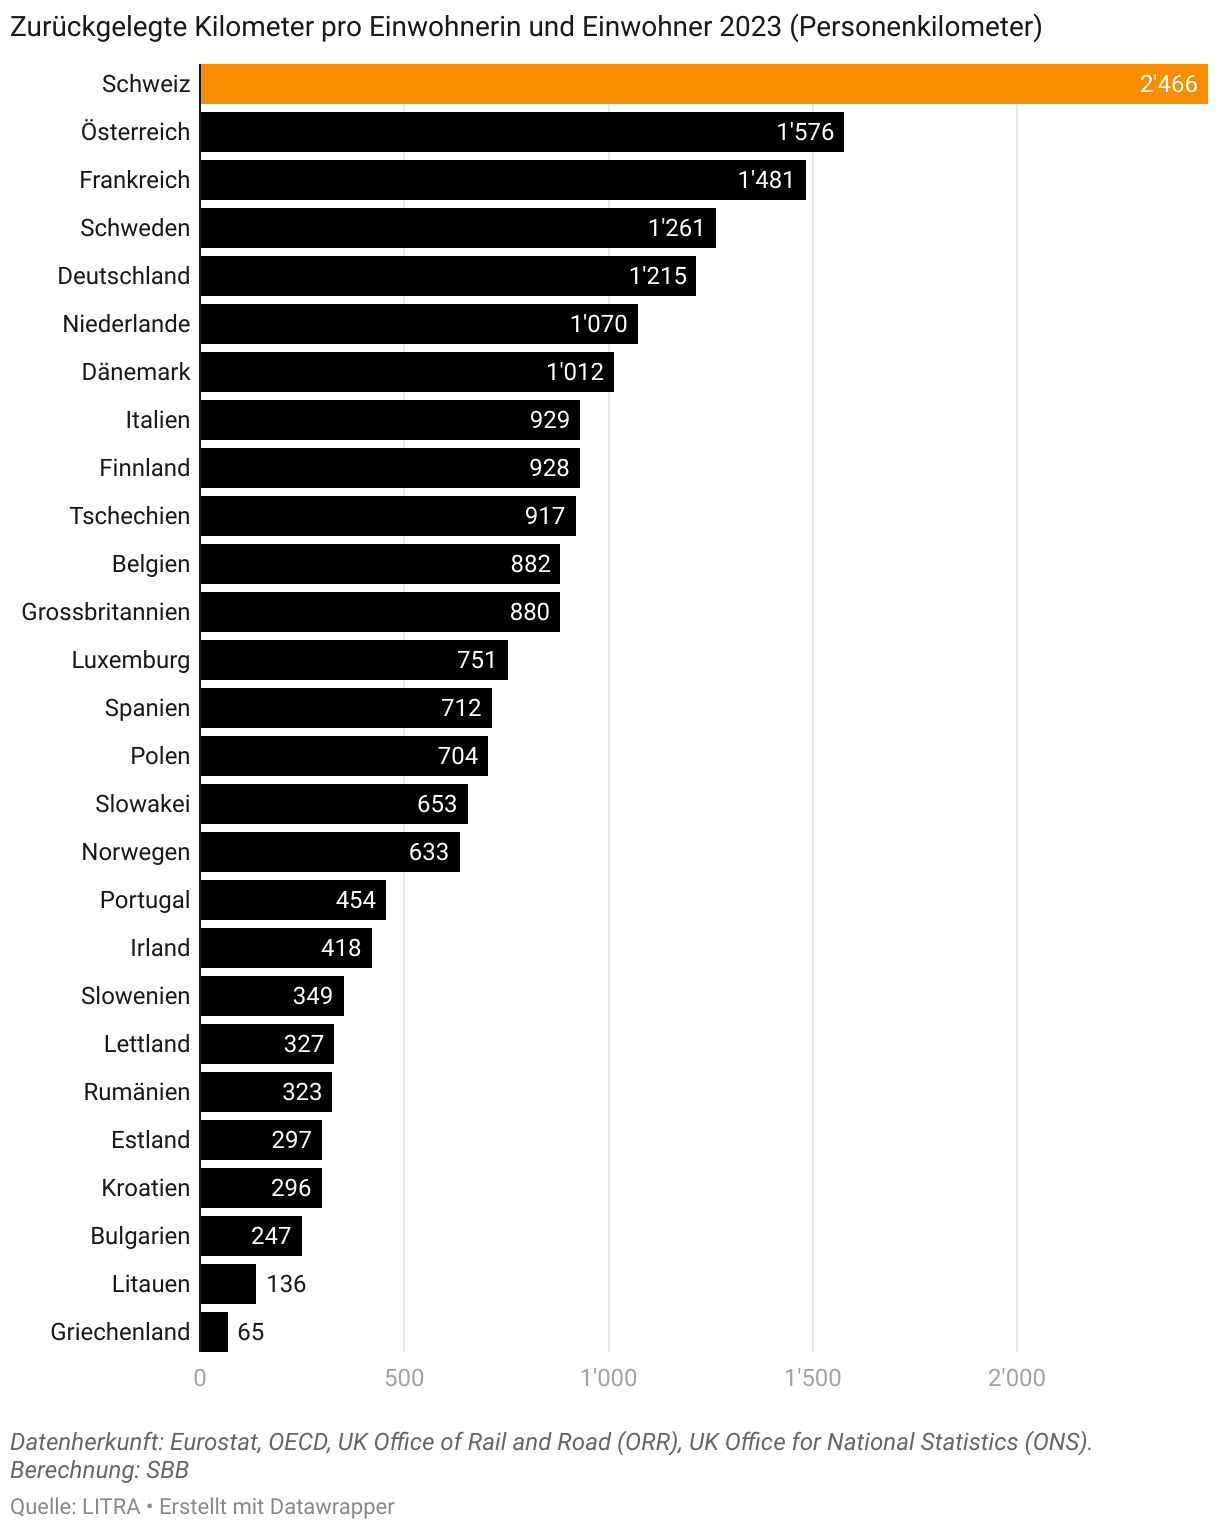
\includegraphics[width=.4\linewidth]{content/00_assets/schweizer_fahren_zug.png}
    \label{fig_schweizer_fahren_zug}
\end{figure}

Auch scheint es keine Anzeichen einer Abschwächung der Zugnutzung zu geben, ganz im Gegenteil. Gemäss der \acrfull{sbb} sollen im Jahr 2040 bereits zwei Millionen Menschen pro Tag mit dem Zug fahren, dies entspricht einer Zunahme von rund 30 Prozent \parencite{sbb_ausbauschritt_2025}.

Schaut man sich die Zahlen und Fakten für das SBB-Zugverkehrsnetz aus dem Jahr 2024 an, ergeben sich beachtliche Werte. Täglich werden rund 1.4 Millionen Menschen mithilfe von 11'569 Zügen transportiert. Um das Zugnetz der SBB auf Stand zu halten, werden rund 20'000 Baustellen pro Jahr betrieben. Um es mit den Worten der SBB auszudrücken, sind sowohl das Bauen als auch das Fahren eine Herausforderung \parencite[S.8 - 9]{sbb_geschäftsbericht_2024}. Insbesondere das Fahren nicht nur eine Herausforderung für die Zugnetzbetreiber, sondern auch für die Passagiere, primär dann, wenn Verspätungen involviert sind.

Die vorliegende Arbeit hat sich zum Ziel gesetzt, visuelle Muster und Anomalien im SBB-Zugverkehrsnetzwerk zu explorieren. Hierzu soll ein Visual Analytics Tool entworfen werden. Im Fokus der Arbeit stehen primär Zugverspätungen und deren Auswirkungen. Nebst der eigentlichen Visualisierung der Daten sind auch die dahinterliegenden Algorithmen von grosser Bedeutung. Diese sollen dabei helfen, visuelle Muster auf anschauliche Weise zugänglich zu machen.


    \chapter{Literaturübersicht}
\label{kap:literaturübersicht}

    \chapter{Forschungsfragen}
\label{kap:forschungsfragen}
TODO
    \chapter{Forschungsdesign}
\label{kap:forschungsdesign}
Das Hauptziel der Arbeit ist das Erstellen eines Visual-Analytics-Tools, mithilfe dessen Trends und Anomalien aufgrund von Verspätungen im \acrshort{sbb} Zugnetzwerk exploriert werden können. Das Vorgehen orientiert sich hierbei an der Visualisierungspipeline von Chen et al. (siehe Abbildung \ref{fig_pipeline_traffic_visualization}), fügt jedoch noch zusätzliche Schritte wie UI-Design, Algorithmen sowie Performance-Analyse hinzu (siehe Abbildung \ref{fig_vorgehen}). Der Entwicklungsfortschritt des Tools wird laufend mit dem Hauptbetreuer der Arbeit reflektiert.

\begin{figure}[H]
    \caption{Vorgehensweise (eigene Darstellung)}
    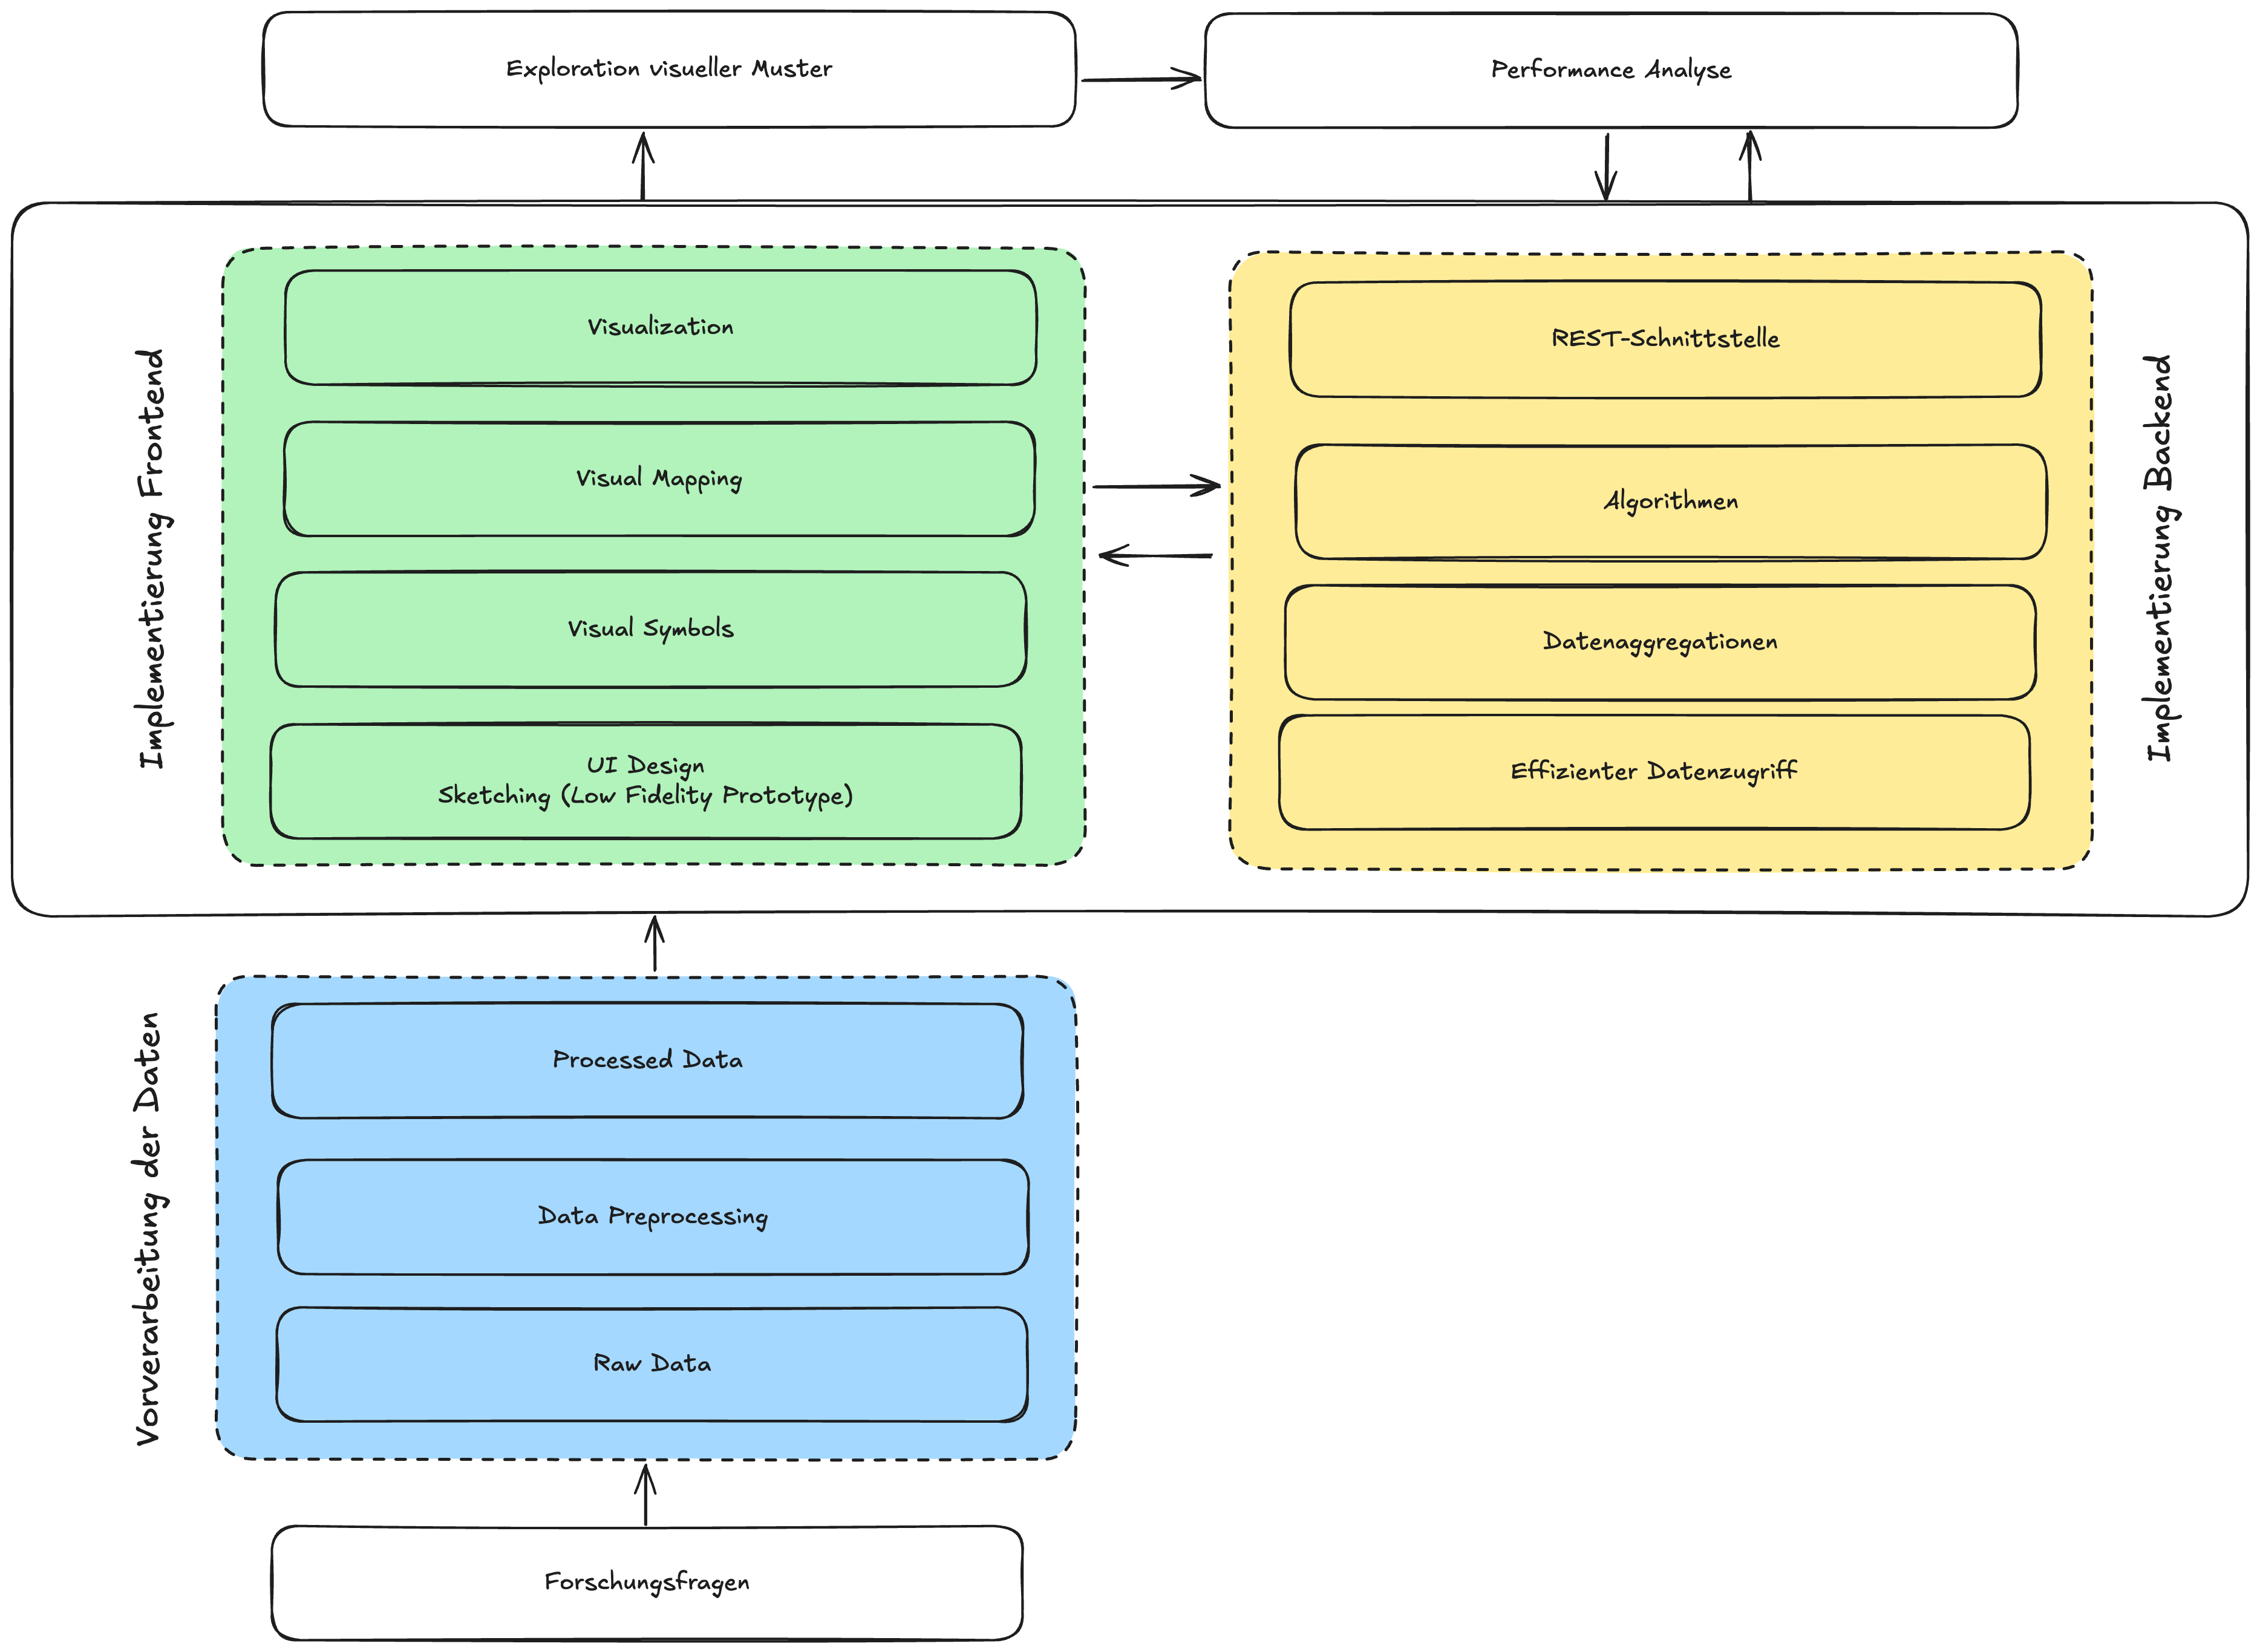
\includegraphics[width=.8\linewidth]{content/00_assets/vorgehen.png}
    \label{fig_vorgehen}
\end{figure}


Das VA-Tool selbst wird aus drei Hauptbestandteilen aufgebaut, einem \textbf{Frontend}, einem \textbf{Backend}, sowie einer \textbf{\acrfull{rest} API}. Das \textbf{Frontend} ist für die Visualisierung der Daten sowie die Handhabung der Nutzerinteraktionen zuständig. Das \textbf{Backend} ist für die notwendigen Algorithmen und die Datenabfragen verantwortlich. Das Frontend und Backend kommunizieren miteinander über eine  \acrshort{rest} Schnittstelle (siehe Abbildung \ref{fig_va_tool_design}). Diese Trennung hat den Vorteil, dass die Visualisierungslogik von der Anwenderlogik getrennt ist und somit die Visualisierungslogik unabhängig von der Anwendungslogik ausgetauscht werden kann.

\begin{figure}[H]
    \caption{Technischer Aufbau des Visual Analytic Tools (eigene Darstellung)}
    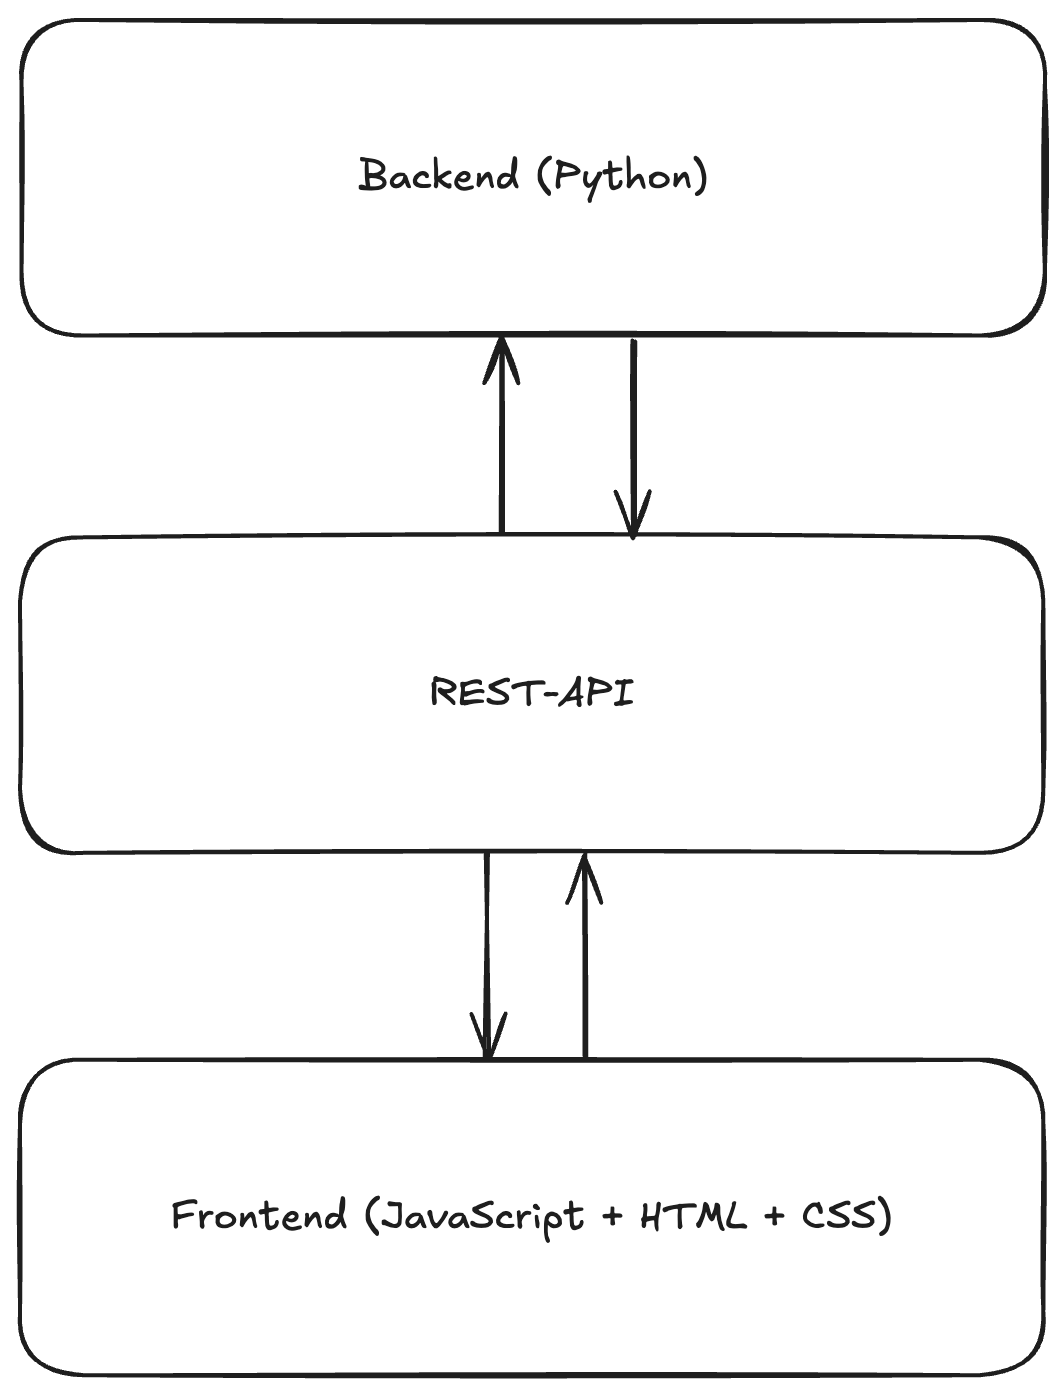
\includegraphics[width=.3\linewidth]{content/00_assets/aufbau_va_tool.png}
    \label{fig_va_tool_design}
\end{figure}

Nachfolgend wird auf die wichtigsten Elemente gemäss Abbildung \ref{fig_vorgehen} eingegangen.

\section{Vorverarbeitung der Daten}
Ausgehend von den Forschungsfragen werden die Datenquellen evaluiert und entsprechend aufbereitet.

\subsection{Raw Data}
Als Datengrundlage dienen die öffentlich zugänglichen Daten der SBB auf Open Data\footnote{\url{https://data.sbb.ch/pages/home/}}. Als Hauptdatenquelle wird die Gegenüberstellung von Zielankunftszeit zu den effektiven Ankunftszeiten verwendet\footnote{\url{https://data.sbb.ch/explore/dataset/actual-data-sbb-previous-day/information/}}. Hieraus lassen sich die Verspätungen pro Station und Zuglinie ermitteln. Als weitere Datenquellen wird das Betriebspunktenetz\footnote{\url{https://data.sbb.ch/explore/dataset/linie-mit-betriebspunkten/information/}} verwendet. Weitere Datenquellen werden im Verlaufe der Arbeit, soweit sinnvoll, hinzugenommen.

\subsection{Data Preprocessing}
Innerhalb des Data Preprocessing werden die Daten optimal zur Beantwortung der Forschungsfragen aufbereitet. Hierunter fallen insbesondere das Data Cleaning sowie notwendige Daten-Aggregationen. Um sicherzustellen, dass auf einfache Art und Weise neue Datensätze eingebunden werden können, wird ein entsprechendes Python-Script geschrieben, welches das Data Preprocessing automatisiert.

\subsection{Processed Data}
Die vorverarbeiteten Daten werden optimal für einen schnellen Zugriff gespeichert. Falls notwendig, werden  Datenbanksysteme speziell für analytische Datenauswertungen wie DuckDB verwendet.

\section{Implementierung Frontend und Backend}
Sowohl Frontend und Backend werden parallel entwickelt. Dies ist notwendig, um die Daten, welche das Backend liefert, dem Nutzer zu visualisieren, als auch um auf bestimmte Nutzerinteraktionen (Filterung, Anpassung der Parameter) zu reagieren und gegebenenfalls die Algorithmen anzupassen.

\subsection{Frontend}
Ausgehend von den Forschungsfragen sowie den vorverarbeiteten Daten wird ein Low Fidelity Prototyp des Tools in Form einer Skizze erstellt. Aufgrund der Skizze werden anschliessend die Visual Symbols (Liniendiagramme etc.) umgesetzt. Um möglichst viele Endnutzer zu erreichen und einen einfachen Zugriff zu ermöglichen, wird das Frontend als Web-Applikation mittels JavaScript, HTML und CSS entwickelt.

\subsection{Backend}
Das Backend beinhaltet die komplette Algorithmik und ist für einen effizienten Datenzugriff und entsprechende Datenaggregation zuständig. Bei den Algorithmen werden verschiedene Cluster-Algorithmen evaluiert (bspw. K-Means für räumliches Clustering). Teil des Backends ist auch die Implementierung einer \acrshort{rest} Schnittstelle.

\section{Exploration visueller Muster und Performance Analyse}
Nachdem das Frontend sowie Backend erstellt wurden, können die visuellen Muster mithilfe des Tools exploriert werden. Um eine effiziente Exploration zu ermöglichen, wird auch eine Performance-Analyse durchgeführt, was wiederum Anpassungen am Front- sowie Backend mit sich führen kann.

    \chapter{Meilensteine und Zeitplan}
\label{kap:meilensteine_zeitplan}
Die Meilensteine wurden aufgrund des beschriebenen Vorgehens in Kapitel \ref{kap:forschungsdesign} definiert. Der Hauptteil der Masterarbeit besteht in der Implementierung eines VA-Tools. Anschliessend sollen Trends und Anomalien im Zugnetzwerk der \acrshort{sbb} mithilfe des entwickelten Tools exploriert werden. Für die Entwicklung des VA-Tools sind die Meilensteine M0 bis M2 vorgesehen. Wie bereits in Kapitel \ref{kap:forschungsdesign} erwähnt, wird das VA-Tool als Web-Applikation (Frontend, Backend und \acrshort{rest}-Schnittstelle) umgesetzt. Das Explorieren der Daten mithilfe des Tools erfolgt im Meilenstein M3. Dem Autor ist es zudem wichtig, ein skalierbares VA-Tool zu entwickeln. Dies wird mithilfe des Meilensteins M4 sichergestellt (siehe Tabelle \ref{table:meilensteine}). Eine detaillierte Beschreibung zu den einzelnen Aufgaben pro Meilenstein kann dem Zeitplan im Anhang \ref{attachment:zeitplan} entnommen werden.

\begin{table}[ht]
    \caption{Übersicht der Meilensteine}
    \begin{tabularx}{\textwidth} {
        >{\raggedright\arraybackslash}X 
        >{\raggedright\arraybackslash}X}
            \hline
            \textbf{Meilenstein} & \textbf{Datum} \\
            \hline
            M0: Datenvorverarbeitung     & 18.05.2025     \\
            M1: Implementierung Frontend & 15.06.2025     \\
            M2: Implementierung Backend  & 15.06.2025     \\
            M3: Anwendung VA-Tool        & 29.06.2025     \\
            M4: Performance Analyse      & 13.07.2025     \\
            M5: Abschluss Masterarbeit   & 25.07.2025     \\
            \hline
    \end{tabularx}
    \bigbreak
    \label{table:meilensteine}
\end{table}




    % Ende Textteil
    
    % Start Nachspann
    \printbibliography[heading=bibintoc,title={Literaturverzeichnis}]
    \include{content/03_nachspann/hilfsmittelverzeichnis}
    \appendix
    \chapter{Anhang}

    \include{content/03_nachspann/eiderklaerung}
    % Ende Nachspann
    
\end{document}